\newpage

\begin{center}
    \Huge{\textbf{\underline{Exercise 3}}}
\end{center}

\vspace{0.3cm}

For each instruction, provide the corresponding grammar:  
\begin{itemize}
    \item Affectation, where the right-hand side is an arithmetic expression with
        optional parenthesis. 
    \item An `if` statement with an optional `else`.  
    \item A `while` loop.  
    \item A `switch-case` statement.  
\end{itemize}

\vspace{1cm}

\textbf{\underline{\Large{Solution}} :}\\[0.4cm]
\textbf{\underline{Affectation}}\\[0.25cm]
\texttt{<} Affect \texttt{>} \(\to\) Idf = \texttt{<} Exp \texttt{>}\\[0.1cm]
\texttt{<} Exp \texttt{>}\(\to\) Cst \texttt{|} Idf \texttt{|} 
\texttt{<} Exp \texttt{>} + \texttt{<} Exp \texttt{>}
\texttt{|} \texttt{<} Exp \texttt{>} - \texttt{<} Exp \texttt{>}
\texttt{|} \texttt{<} Exp \texttt{>} * \texttt{<} Exp \texttt{>}
\texttt{|} \texttt{<} Exp \texttt{>} / \texttt{<} Exp \texttt{>}
\texttt{|} \texttt{<} Exp \texttt{>} mod \texttt{<} Exp \texttt{>}
\texttt{|} ( \texttt{<} Exp \texttt{>} )

\vspace{1cm}

\textbf{\underline{Tree Examples}}

\begin{center} 
    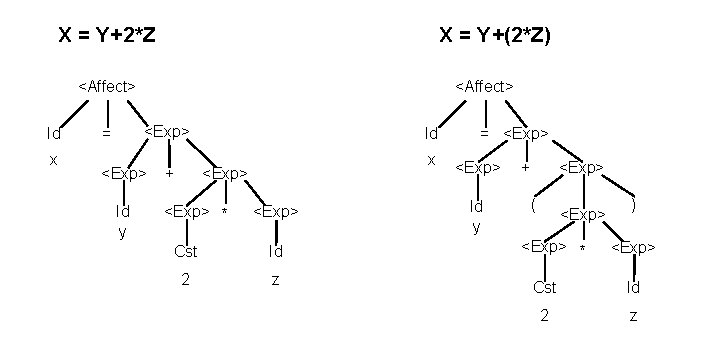
\includegraphics[height=0.5\textheight]{Exercices/EX3/tree3.1.drawio.pdf}
\end{center}

